\chapter{PHÂN TÍCH VÀ THIẾT KẾ HỆ THỐNG}

\section{Kiến trúc hệ thống}
Hệ thống được thiết kế theo hướng pipeline đa module nhằm hỗ trợ phát hiện dấu hiệu rủi ro trong quảng cáo thực phẩm chức năng trên mạng xã hội. Sau giai đoạn thu thập và chuẩn hóa dữ liệu, các mô hình phát hiện được tổ chức thành những lớp xử lý độc lập, chạy song song để tạo điểm dự đoán riêng. Tầng hợp nhất ở cuối pipeline nhận kết quả từ từng lớp mô hình và tạo nhãn, xác suất, bằng chứng cùng điểm rủi ro tổng hợp. Cách thiết kế này giúp hệ thống dễ mở rộng khi cần bổ sung nguồn dữ liệu mới, mô hình mới hoặc nhóm tín hiệu rủi ro mới.

Về tổng thể, hệ thống gồm các lớp chức năng chính sau:
\begin{itemize}
    \item \textbf{Lớp thu thập dữ liệu:} tiếp nhận bài đăng, video, metadata, đường dẫn nguồn và văn bản thô từ các nền tảng như TikTok hoặc Facebook.
    \item \textbf{Lớp xử lý và quản lý dữ liệu:} chuẩn hóa dữ liệu, loại bỏ trùng lặp, quản lý nhãn, chia tập train/validation/test và lưu phiên bản dataset.
    \item \textbf{Lớp rule-based detection:} đọc tập keyword, phát hiện cụm từ rủi ro, xác định nhãn gợi ý và lưu đoạn bằng chứng trong văn bản.
    \item \textbf{Lớp PhoBERT:} suy luận mô hình PhoBERT đã fine-tune cho phân loại đa nhãn và trả về \texttt{phobert\_score} cho từng nhãn.
    \item \textbf{Lớp OCR:} trích xuất frame từ ảnh/video, nhận diện chữ nhúng và tạo \texttt{OCR\_score} dựa trên nội dung chữ nhận diện được.
    \item \textbf{Lớp ASR:} trích xuất audio từ video, chuyển lời nói thành văn bản và tạo \texttt{ASR\_score} từ nội dung transcript.
    \item \textbf{Lớp visual detection:} phát hiện các tín hiệu hình ảnh có rủi ro như áo blouse, ống nghe, phòng khám hoặc hình ảnh chuyên gia y tế và tạo \texttt{visual\_score}.
    \item \textbf{Lớp hợp nhất và chấm điểm rủi ro:} kết hợp điểm từ các lớp chạy song song để tạo điểm rủi ro tổng hợp.
    \item \textbf{Lớp truy xuất và giải thích:} truy xuất quy định, nguyên tắc gán nhãn và bằng chứng liên quan để hỗ trợ sinh kết luận có giải thích.
    \item \textbf{Lớp API/Demo:} cung cấp chức năng dự đoán cho người dùng hoặc hệ thống bên ngoài, trả về nhãn, xác suất, bằng chứng và phần giải thích.
\end{itemize}

Luồng xử lý chính của hệ thống bắt đầu từ việc thu thập bài đăng hoặc video. Dữ liệu thô sau đó được chuẩn hóa và kiểm tra chất lượng trước khi đưa vào các lớp mô hình song song. Văn bản từ caption hoặc mô tả được đưa đồng thời vào rule-based detection và PhoBERT. Hình ảnh hoặc video được đưa đồng thời vào OCR, ASR và visual detection. Mỗi lớp trả về score, nhãn gợi ý và bằng chứng tương ứng; tầng fusion tiếp nhận các kết quả này để tạo nhãn dự đoán, xác suất cuối cùng và điểm rủi ro. Cuối cùng, hệ thống có thể sử dụng module RAG và LLM reasoning để sinh phần giải thích phục vụ rà soát thủ công.

\begin{figure}[H]
\centering
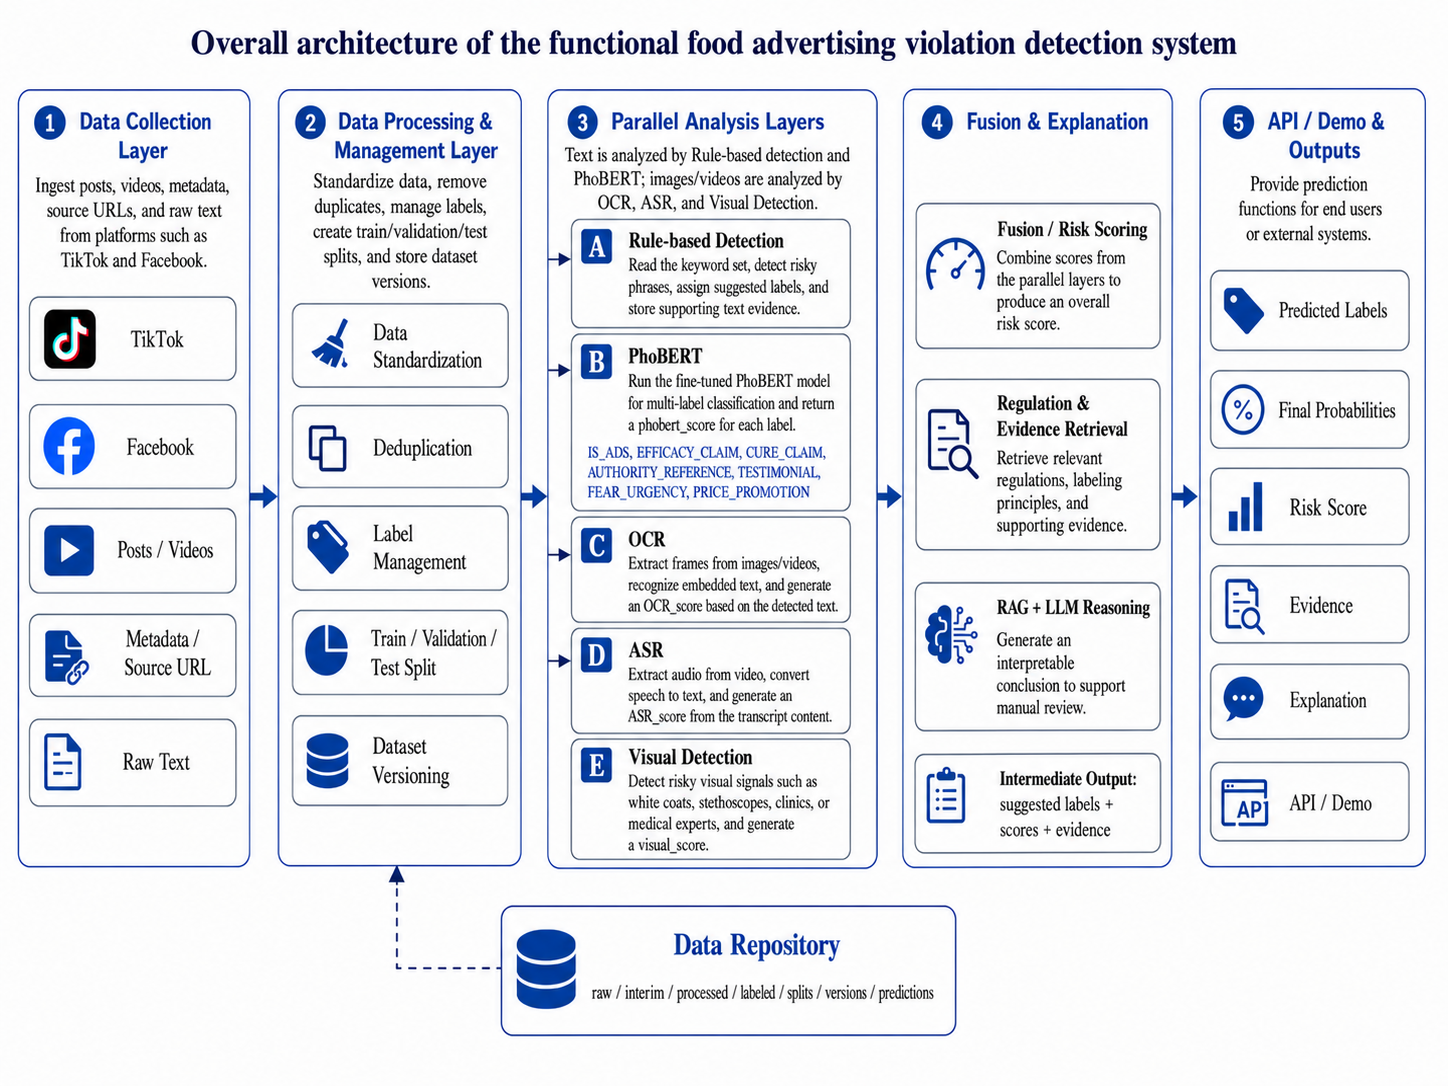
\includegraphics[width=\textwidth]{images/OveralArchitecture.png}
\caption{Kiến trúc tổng thể của hệ thống phát hiện dấu hiệu sai phạm trong quảng cáo thực phẩm chức năng}
\label{fig:overall_architecture}
\end{figure}

\section{Thiết kế UC}
Thiết kế UC mô tả các chức năng chính mà người dùng hoặc thành phần bên ngoài có thể tương tác với hệ thống. Các tác nhân chính gồm người quản trị dữ liệu, người gán nhãn hoặc rà soát, người dùng demo/API và các module AI nội bộ của hệ thống. Danh sách use case chính gồm:

\begin{itemize}
    \item \textbf{UC01 -- Thu thập dữ liệu:} người quản trị dữ liệu thu thập bài đăng, video, metadata, đường dẫn nguồn và văn bản thô từ TikTok hoặc Facebook.
    \item \textbf{UC02 -- Xử lý và chuẩn hóa dữ liệu:} người quản trị dữ liệu chuẩn hóa dữ liệu, kiểm tra duplicate bằng Python, tải media bằng \texttt{yt-dlp} và trích frame bằng \texttt{FFmpeg}.
    \item \textbf{UC03 -- Quản lý và gán nhãn dữ liệu:} người gán nhãn sử dụng AI để hỗ trợ gán nhãn văn bản, trích evidence, review nhiều vòng và dùng Roboflow để gán nhãn hình ảnh.
    \item \textbf{UC04 -- Chia tập và lưu phiên bản dataset:} người quản trị dữ liệu chia dữ liệu thành train, validation và test, lưu thông tin phiên bản dataset và thống kê phân phối nhãn.
    \item \textbf{UC05 -- Phát hiện rủi ro bằng luật:} module rule-based đọc keyword, phát hiện cụm từ rủi ro, trả về nhãn gợi ý và evidence span trong văn bản.
    \item \textbf{UC06 -- Huấn luyện mô hình PhoBERT:} người nghiên cứu huấn luyện PhoBERT trên tập train, chọn checkpoint tốt nhất và lưu mô hình.
    \item \textbf{UC07 -- Suy luận văn bản bằng PhoBERT:} lớp PhoBERT dự đoán xác suất cho từng nhãn từ văn bản đầu vào.
    \item \textbf{UC08 -- Phân tích ảnh và video:} các lớp OCR, ASR và visual detection chạy song song để nhận diện chữ, lời nói và tín hiệu hình ảnh rủi ro.
    \item \textbf{UC09 -- Hợp nhất điểm rủi ro:} module fusion kết hợp phobert score, OCR score, ASR score, visual score và rule score để tạo risk score tổng hợp.
    \item \textbf{UC10 -- Truy xuất quy định và sinh giải thích:} module RAG/LLM truy xuất quy định, nguyên tắc gán nhãn, bằng chứng liên quan và sinh phần giải thích cho kết quả dự đoán.
    \item \textbf{UC11 -- Dự đoán qua API hoặc demo:} người dùng demo/API gửi văn bản hoặc metadata bài đăng tới endpoint dự đoán, nhận nhãn, xác suất, bằng chứng và giải thích.
    \item \textbf{UC12 -- Xuất kết quả phục vụ rà soát:} người rà soát xuất file kết quả gồm dữ liệu, nhãn thật, nhãn dự đoán, xác suất, điểm rủi ro và ghi chú lỗi để kiểm tra thủ công.
\end{itemize}

\subsection{Đặc tả UC01 -- Thu thập dữ liệu}
UC01 mô tả chức năng thu thập dữ liệu thô từ TikTok/Facebook thông qua Apify và lưu trữ kết quả trên Google Drive. Đây là use case đầu vào của toàn bộ pipeline, vì chất lượng dữ liệu thu thập ảnh hưởng trực tiếp đến các bước xử lý, gán nhãn và huấn luyện mô hình phía sau.

\begin{figure}[H]
\centering
\resizebox{\textwidth}{!}{
\begin{tikzpicture}[
    font=\footnotesize,
    actor/.style={
        rectangle,
        rounded corners=3pt,
        draw,
        thick,
        align=center,
        text width=2.7cm,
        minimum height=1.05cm,
        fill=white
    },
    usecase/.style={
        ellipse,
        draw,
        thick,
        align=center,
        text width=4.2cm,
        minimum height=1.05cm,
        fill=white
    },
    boundary/.style={
        rectangle,
        rounded corners=6pt,
        draw,
        dashed,
        inner xsep=18pt,
        inner ysep=16pt
    },
    link/.style={-{Latex[length=2.3mm]}, thick, shorten >=2pt, shorten <=2pt},
    assoc/.style={thick}
]
\node[actor] (admin) at (-3.3,3.20) {Người quản trị\\dữ liệu};
\node[actor] (apify) at (9.6,-1.10) {Apify};
\node[actor] (platform) at (9.6,0.85) {TikTok /\\Facebook};
\node[actor] (drive) at (9.6,-4.30) {Google Drive};

\node[usecase] (config) at (3.0,4.30) {Cấu hình\\tác vụ Apify};
\node[usecase] (input) at (3.0,2.15) {Nhập từ khóa\\hoặc URL};
\node[usecase] (crawl) at (3.0,0.00) {Thu thập\\bài đăng/video};
\node[usecase] (extract) at (3.0,-2.15) {Trích xuất text thô\\và metadata};
\node[usecase] (save) at (3.0,-4.30) {Lưu dữ liệu thô\\lên Google Drive};

\node[boundary, fit=(config)(input)(crawl)(extract)(save)] (system) {};
\node[fill=white, font=\bfseries] at (system.north) {UC01 -- Thu thập dữ liệu};

\draw[link] (admin.north east) -- (config.west);
\draw[link] (admin.south east) -- (input.west);
\draw[link] (config.south) -- (input.north);
\draw[link] (input.south) -- (crawl.north);
\draw[link] (crawl.south) -- (extract.north);
\draw[link] (extract.south) -- (save.north);
\draw[link] (config.east) -- (apify.north west);
\draw[link] (platform.south) -- (apify.north);
\draw[link] (apify.west) -- (crawl.south east);
\draw[link] (apify.south west) -- (extract.north east);
\draw[link] (save.east) -- (drive.west);
\end{tikzpicture}
}
\caption{Use case UC01 -- Thu thập dữ liệu}
\label{fig:uc01_data_collection}
\end{figure}

\begin{longtable}{|p{0.25\textwidth}|p{0.65\textwidth}|}
\caption{Đặc tả use case UC01 -- Thu thập dữ liệu}\\
\hline
\textbf{Thành phần} & \textbf{Nội dung} \\
\hline
\endfirsthead
\hline
\textbf{Thành phần} & \textbf{Nội dung} \\
\hline
\endhead
Mã use case & UC01 \\ \hline
Tên use case & Thu thập dữ liệu \\ \hline
Tác nhân chính & Người quản trị dữ liệu \\ \hline
Tác nhân phụ & Apify, TikTok/Facebook, Google Drive \\ \hline
Mục tiêu & Thu thập bài đăng, video, metadata, source URL, file/video link và văn bản thô từ TikTok/Facebook thông qua Apify, sau đó lưu dữ liệu thô lên Google Drive để phục vụ xử lý, gán nhãn và huấn luyện mô hình. \\ \hline
Tiền điều kiện & Người quản trị dữ liệu đã xác định nền tảng, từ khóa, nhóm sản phẩm hoặc danh sách URL cần thu thập; tác vụ Apify đã sẵn sàng để chạy. \\ \hline
Hậu điều kiện & Dữ liệu thô được lưu trên Google Drive, bao gồm raw text, metadata, source URL, file/video link, nền tảng và định danh mẫu dữ liệu. \\ \hline
Luồng chính &
\begin{minipage}[t]{\linewidth}
\begin{enumerate}[label=\textbf{Bước \arabic*:}, leftmargin=1.55cm, itemsep=0pt, topsep=0pt]
    \item Người quản trị dữ liệu cấu hình tác vụ Apify.
    \item Người quản trị nhập từ khóa, nhóm sản phẩm hoặc URL bài đăng/video.
    \item Apify truy xuất bài đăng/video từ nền tảng nguồn.
    \item Hệ thống nhận kết quả crawl từ Apify.
    \item Hệ thống trích xuất hoặc chuẩn hóa text thô, metadata, source URL và file/video link.
    \item Hệ thống lưu dữ liệu thô lên Google Drive.
    \item Hệ thống trả về trạng thái thu thập thành công.
\end{enumerate}
\end{minipage} \\ \hline
Luồng thay thế &
\begin{minipage}[t]{\linewidth}
\begin{enumerate}[label=\textbf{Bước \arabic*:}, leftmargin=1.55cm, itemsep=0pt, topsep=0pt]
    \item Nếu URL không hợp lệ, bài đăng/video không truy cập được hoặc Apify trả lỗi, hệ thống ghi nhận lỗi và bỏ qua mẫu đó.
    \item Nếu dữ liệu đã tồn tại trên Google Drive, hệ thống đánh dấu trùng lặp để xử lý ở bước sau.
\end{enumerate}
\end{minipage} \\ \hline
Dữ liệu đầu vào & Từ khóa, nhóm sản phẩm, URL bài đăng/video, nền tảng và cấu hình tác vụ Apify. \\ \hline
Dữ liệu đầu ra & Dữ liệu thô trên Google Drive gồm raw text, source URL, file/video link, platform, post/video id, thời gian thu thập và metadata liên quan. \\ \hline
Ngoại lệ & Apify lỗi, hết quota, URL lỗi, bài đăng/video bị xóa, nội dung bị giới hạn quyền truy cập, thiếu metadata hoặc không lưu được lên Google Drive. \\ \hline
\end{longtable}

\subsection{Đặc tả UC02 -- Xử lý và chuẩn hóa dữ liệu}
UC02 mô tả chức năng xử lý dữ liệu thô sau khi thu thập. Hệ thống đọc dữ liệu từ Google Drive, chuẩn hóa văn bản và metadata, kiểm tra dữ liệu trùng lặp bằng Python, tải ảnh/video bằng \texttt{yt-dlp}, cắt video thành frame bằng \texttt{FFmpeg} và chỉ giữ các frame liên tiếp có độ khác biệt lớn hơn 70\%. Kết quả của UC02 là bộ dữ liệu sạch hơn, có cấu trúc rõ hơn và sẵn sàng cho các bước gán nhãn, huấn luyện hoặc phân tích ảnh/video.

\begin{figure}[H]
\centering
\resizebox{\textwidth}{!}{
\begin{tikzpicture}[
    font=\footnotesize,
    actor/.style={
        rectangle,
        rounded corners=3pt,
        draw,
        thick,
        align=center,
        text width=2.7cm,
        minimum height=1.05cm,
        fill=white
    },
    usecase/.style={
        ellipse,
        draw,
        thick,
        align=center,
        text width=4.35cm,
        minimum height=1.05cm,
        fill=white
    },
    boundary/.style={
        rectangle,
        rounded corners=6pt,
        draw,
        dashed,
        inner xsep=18pt,
        inner ysep=16pt
    },
    link/.style={-{Latex[length=2.3mm]}, thick, shorten >=2pt, shorten <=2pt}
]
\node[actor] (admin2) at (-3.6,6.20) {Người quản trị\\dữ liệu};
\node[actor] (driveRaw) at (10.0,5.05) {Google Drive\\dữ liệu thô};
\node[actor] (python) at (10.0,1.45) {Python};
\node[actor] (ytdlp) at (10.0,-2.15) {\texttt{yt-dlp}};
\node[actor] (ffmpeg) at (10.0,-4.15) {\texttt{FFmpeg}};
\node[actor] (driveClean) at (10.0,-7.05) {Google Drive\\dữ liệu xử lý};

\node[usecase] (cfg2) at (3.0,7.00) {Cấu hình\\quy trình xử lý};
\node[usecase] (read2) at (3.0,5.00) {Đọc dữ liệu thô\\từ Google Drive};
\node[usecase] (norm2) at (3.0,3.00) {Chuẩn hóa text\\và metadata};
\node[usecase] (dup2) at (3.0,1.00) {Kiểm tra duplicate\\bằng Python};
\node[usecase] (download2) at (3.0,-1.00) {Tải ảnh/video\\bằng \texttt{yt-dlp}};
\node[usecase] (frame2) at (3.0,-3.00) {Cắt video\\thành frame};
\node[usecase] (filter2) at (3.0,-5.00) {Lọc frame khác biệt\\lớn hơn 70\%};
\node[usecase] (save2) at (3.0,-7.00) {Lưu dữ liệu\\đã xử lý};

\node[boundary, fit=(cfg2)(read2)(norm2)(dup2)(download2)(frame2)(filter2)(save2)] (system2) {};
\node[fill=white, font=\bfseries] at (system2.north) {UC02 -- Xử lý và chuẩn hóa dữ liệu};

\draw[link] (admin2.north east) -- (cfg2.west);
\draw[link] (admin2.south east) -- (read2.west);
\draw[link] (cfg2.south) -- (read2.north);
\draw[link] (read2.south) -- (norm2.north);
\draw[link] (norm2.south) -- (dup2.north);
\draw[link] (dup2.south) -- (download2.north);
\draw[link] (download2.south) -- (frame2.north);
\draw[link] (frame2.south) -- (filter2.north);
\draw[link] (filter2.south) -- (save2.north);
\draw[link] (driveRaw.west) -- (read2.east);
\draw[link] (dup2.east) -- (python.west);
\draw[link] (filter2.east) -- (python.south west);
\draw[link] (download2.east) -- (ytdlp.west);
\draw[link] (frame2.east) -- (ffmpeg.west);
\draw[link] (save2.east) -- (driveClean.west);
\end{tikzpicture}
}
\caption{Use case UC02 -- Xử lý và chuẩn hóa dữ liệu}
\label{fig:uc02_data_processing}
\end{figure}

\begin{longtable}{|p{0.25\textwidth}|p{0.65\textwidth}|}
\caption{Đặc tả use case UC02 -- Xử lý và chuẩn hóa dữ liệu}\\
\hline
\textbf{Thành phần} & \textbf{Nội dung} \\
\hline
\endfirsthead
\hline
\textbf{Thành phần} & \textbf{Nội dung} \\
\hline
\endhead
Mã use case & UC02 \\ \hline
Tên use case & Xử lý và chuẩn hóa dữ liệu \\ \hline
Tác nhân chính & Người quản trị dữ liệu \\ \hline
Tác nhân phụ & Google Drive, Python, \texttt{yt-dlp}, \texttt{FFmpeg} \\ \hline
Mục tiêu & Chuẩn hóa dữ liệu thô sau thu thập, kiểm tra duplicate, tải media, cắt video thành frame và lưu lại dữ liệu đã xử lý để phục vụ gán nhãn, huấn luyện và phân tích đa phương thức. \\ \hline
Tiền điều kiện & Dữ liệu thô đã được lưu trên Google Drive; các trường như raw text, metadata, source URL và file/video link đã có ở mức tối thiểu; môi trường xử lý đã cài Python, \texttt{yt-dlp} và \texttt{FFmpeg}. \\ \hline
Hậu điều kiện & Dữ liệu đã được chuẩn hóa, mẫu trùng lặp được đánh dấu hoặc loại bỏ, media cần thiết được tải về, video được tách frame và các frame được lọc theo ngưỡng khác biệt lớn hơn 70\%. \\ \hline
Luồng chính &
\begin{minipage}[t]{\linewidth}
\begin{enumerate}[label=\textbf{Bước \arabic*:}, leftmargin=1.55cm, itemsep=0pt, topsep=0pt]
    \item Người quản trị dữ liệu cấu hình quy trình xử lý dữ liệu.
    \item Hệ thống đọc dữ liệu thô từ Google Drive.
    \item Hệ thống chuẩn hóa văn bản, metadata, source URL, định dạng thời gian và định danh mẫu.
    \item Hệ thống sử dụng Python để kiểm tra duplicate theo nội dung, URL, post/video id hoặc metadata liên quan.
    \item Hệ thống dùng \texttt{yt-dlp} để tải ảnh/video từ các link hợp lệ khi cần xử lý media.
    \item Hệ thống dùng \texttt{FFmpeg} để cắt video thành các frame liên tiếp.
    \item Hệ thống so sánh các frame liên tiếp và chỉ giữ frame có độ khác biệt lớn hơn 70\% so với frame trước đó.
    \item Hệ thống lưu dữ liệu đã xử lý, log lỗi, danh sách duplicate và đường dẫn frame/media lên Google Drive.
\end{enumerate}
\end{minipage} \\ \hline
Luồng thay thế &
\begin{minipage}[t]{\linewidth}
\begin{enumerate}[label=\textbf{Bước \arabic*:}, leftmargin=1.55cm, itemsep=0pt, topsep=0pt]
    \item Nếu bản ghi bị thiếu text hoặc metadata quan trọng, hệ thống đánh dấu trạng thái cần kiểm tra thủ công.
    \item Nếu URL media không tải được bằng \texttt{yt-dlp}, hệ thống ghi log lỗi và vẫn giữ phần text/metadata đã chuẩn hóa.
    \item Nếu video lỗi hoặc \texttt{FFmpeg} không trích được frame, hệ thống bỏ qua nhánh frame và ghi lý do lỗi.
    \item Nếu các frame liên tiếp có độ khác biệt không vượt quá 70\%, hệ thống loại frame sau để giảm trùng lặp hình ảnh.
\end{enumerate}
\end{minipage} \\ \hline
Dữ liệu đầu vào & Dữ liệu thô trên Google Drive gồm raw text, metadata, source URL, file/video link, platform, post/video id và thời gian thu thập. \\ \hline
Dữ liệu đầu ra & Dữ liệu đã chuẩn hóa, danh sách duplicate, file media đã tải, frame đã lọc, log lỗi và metadata cập nhật. \\ \hline
Quy tắc xử lý & Duplicate được kiểm tra bằng Python; media được tải bằng \texttt{yt-dlp}; video được cắt bằng \texttt{FFmpeg}; chỉ giữ frame khi độ khác biệt với frame liền trước lớn hơn 70\%. \\ \hline
Ngoại lệ & Thiếu trường dữ liệu bắt buộc, URL hỏng, media bị giới hạn quyền truy cập, \texttt{yt-dlp}/\texttt{FFmpeg} lỗi, không đủ dung lượng lưu trữ hoặc không ghi được kết quả lên Google Drive. \\ \hline
\end{longtable}

\subsection{Đặc tả UC03 -- Quản lý và gán nhãn dữ liệu}
UC03 mô tả quy trình gán nhãn dữ liệu sau khi dữ liệu đã được chuẩn hóa ở UC02. Với dữ liệu văn bản, hệ thống sử dụng AI để chia các đoạn dài thành nhiều đoạn nhỏ đủ phù hợp với đầu vào của PhoBERT, gắn \texttt{post\_id} để tránh leakage khi chia train/validation/test, hỗ trợ gán nhãn và trích evidence dựa trên tập \texttt{keyword.json}. Kết quả gán nhãn văn bản được người rà soát kiểm tra lại và quy trình này được lặp ba lần để tăng độ tin cậy của dữ liệu. Với dữ liệu hình ảnh, Roboflow được sử dụng làm nền tảng chính để quản lý dataset, tạo model từ các dataset liên quan đến nhãn cần thiết, thêm các frame đã cắt ở UC02, auto label và review annotation.

\begin{figure}[H]
\centering
\resizebox{\textwidth}{!}{
\begin{tikzpicture}[
    font=\footnotesize,
    actor/.style={
        rectangle,
        rounded corners=3pt,
        draw,
        thick,
        align=center,
        text width=2.9cm,
        minimum height=1.05cm,
        fill=white
    },
    usecase/.style={
        ellipse,
        draw,
        thick,
        align=center,
        text width=3.25cm,
        minimum height=1.05cm,
        fill=white
    },
    boundary/.style={
        rectangle,
        rounded corners=6pt,
        draw,
        dashed,
        inner xsep=18pt,
        inner ysep=16pt
    },
    link/.style={-{Latex[length=2.3mm]}, thick, shorten >=2pt, shorten <=2pt}
]
\node[actor] (reviewer3) at (-3.8,3.60) {Người gán nhãn\\và rà soát};
\node[actor] (ai3) at (-3.8,1.25) {AI hỗ trợ\\gán nhãn};
\node[actor] (keyword3) at (-3.8,-1.10) {\texttt{keyword.json}};
\node[actor] (relatedData3) at (12.0,4.60) {Dataset hình ảnh\\liên quan};
\node[actor] (roboflow3) at (12.0,1.35) {Roboflow};
\node[actor] (frame3) at (12.0,-0.95) {Frame từ UC02};
\node[actor] (imageReviewer3) at (12.0,-2.85) {Người review\\annotation};
\node[actor] (drive3) at (12.0,-4.70) {Kho dữ liệu\\đã gán nhãn};

\node[usecase] (postid3) at (0.90,4.60) {Gắn \texttt{post\_id}\\chống leakage};
\node[usecase] (chunk3) at (0.90,2.85) {Chia text dài\\thành đoạn nhỏ};
\node[usecase] (labelText3) at (0.90,1.10) {AI gán nhãn text\\và trích evidence};
\node[usecase] (reviewText3) at (0.90,-0.65) {Review nhãn\\văn bản};
\node[usecase] (repeat3) at (0.90,-2.40) {Lặp quy trình\\3 vòng};

\node[usecase] (dataset3) at (6.40,4.60) {Chuẩn bị dataset\\trên Roboflow};
\node[usecase] (model3) at (6.40,2.85) {Tạo model từ\\dataset liên quan};
\node[usecase] (addFrame3) at (6.40,1.10) {Thêm frame\\đã cắt ở UC02};
\node[usecase] (autoLabel3) at (6.40,-0.65) {Auto label\\hình ảnh};
\node[usecase] (reviewImg3) at (6.40,-2.40) {Review\\annotation};

\node[usecase] (save3) at (3.65,-4.60) {Lưu dataset\\đủ tin cậy};

\node[boundary, fit=(postid3)(chunk3)(labelText3)(reviewText3)(repeat3)(dataset3)(model3)(addFrame3)(autoLabel3)(reviewImg3)(save3)] (system3) {};
\node[fill=white, font=\bfseries] at (system3.north) {UC03 -- Quản lý và gán nhãn dữ liệu};

\draw[link] (postid3.south) -- (chunk3.north);
\draw[link] (chunk3.south) -- (labelText3.north);
\draw[link] (labelText3.south) -- (reviewText3.north);
\draw[link] (reviewText3.south) -- (repeat3.north);
\draw[link] (repeat3.south) -- (save3.north west);

\draw[link] (dataset3.south) -- (model3.north);
\draw[link] (model3.south) -- (addFrame3.north);
\draw[link] (addFrame3.south) -- (autoLabel3.north);
\draw[link] (autoLabel3.south) -- (reviewImg3.north);
\draw[link] (reviewImg3.south) -- (save3.north east);

\draw[link] (reviewer3.east) -- (postid3.west);
\draw[link] (reviewer3.south east) -- (reviewText3.west);
\draw[link] (ai3.east) -- (chunk3.west);
\draw[link] (ai3.east) -- (labelText3.west);
\draw[link] (keyword3.east) -- (labelText3.west);
\draw[link] (relatedData3.west) -- (dataset3.east);
\draw[link] (roboflow3.west) -- (model3.east);
\draw[link] (roboflow3.west) -- (autoLabel3.east);
\draw[link] (frame3.west) -- (addFrame3.east);
\draw[link] (imageReviewer3.west) -- (reviewImg3.east);
\draw[link] (save3.east) -- (drive3.west);
\end{tikzpicture}
}
\caption{Use case UC03 -- Quản lý và gán nhãn dữ liệu}
\label{fig:uc03_labeling}
\end{figure}

\begin{longtable}{|p{0.25\textwidth}|p{0.65\textwidth}|}
\caption{Đặc tả use case UC03 -- Quản lý và gán nhãn dữ liệu}\\
\hline
\textbf{Thành phần} & \textbf{Nội dung} \\
\hline
\endfirsthead
\hline
\textbf{Thành phần} & \textbf{Nội dung} \\
\hline
\endhead
Mã use case & UC03 \\ \hline
Tên use case & Quản lý và gán nhãn dữ liệu \\ \hline
Tác nhân chính & Người gán nhãn và rà soát dữ liệu \\ \hline
Tác nhân phụ & AI hỗ trợ gán nhãn, \texttt{keyword.json}, PhoBERT, Roboflow, dataset hình ảnh liên quan, kho frame từ UC02 \\ \hline
Mục tiêu & Tạo bộ dữ liệu văn bản và hình ảnh có nhãn đáng tin cậy, có evidence rõ ràng, hạn chế leakage khi chia tập và sẵn sàng cho huấn luyện mô hình PhoBERT hoặc mô hình thị giác. \\ \hline
Tiền điều kiện & Dữ liệu đã được xử lý ở UC02; văn bản, metadata, \texttt{post\_id}, frame và media liên quan đã có; file \texttt{keyword.json} và workspace Roboflow đã được chuẩn bị. \\ \hline
Hậu điều kiện & Dữ liệu văn bản có nhãn, đoạn evidence và trạng thái review; dữ liệu hình ảnh có annotation đã được kiểm tra; bộ dữ liệu đủ tin cậy sau ba vòng rà soát. \\ \hline
Luồng chính -- văn bản &
\begin{minipage}[t]{\linewidth}
\begin{enumerate}[label=\textbf{Bước \arabic*:}, leftmargin=1.55cm, itemsep=0pt, topsep=0pt]
    \item Hệ thống gắn hoặc kiểm tra \texttt{post\_id} cho từng mẫu để tránh leakage khi chia train/validation/test.
    \item AI hỗ trợ chia các đoạn văn bản dài thành nhiều đoạn nhỏ đủ phù hợp với giới hạn đầu vào của PhoBERT.
    \item AI sử dụng nội dung văn bản và file \texttt{keyword.json} để gợi ý một hoặc nhiều nhãn.
    \item AI trích evidence tương ứng với nhãn, ưu tiên các cụm từ hoặc đoạn văn bản thể hiện rõ dấu hiệu rủi ro.
    \item Người rà soát kiểm tra nhãn, evidence và trạng thái của từng mẫu.
    \item Quy trình gán nhãn và rà soát được lặp lại ba lần để tăng độ tin cậy của dữ liệu.
\end{enumerate}
\end{minipage} \\ \hline
Luồng chính -- hình ảnh &
\begin{minipage}[t]{\linewidth}
\begin{enumerate}[label=\textbf{Bước \arabic*:}, leftmargin=1.55cm, itemsep=0pt, topsep=0pt]
    \item Người rà soát chuẩn bị các dataset hình ảnh liên quan đến các nhãn cần thiết trên Roboflow.
    \item Roboflow được dùng làm nền tảng chính để quản lý dataset và tạo model gán nhãn hình ảnh ban đầu.
    \item Hệ thống thêm các frame đã cắt ở UC02 vào workspace Roboflow.
    \item Roboflow thực hiện auto label cho các hình ảnh/frame mới.
    \item Người rà soát kiểm tra, sửa và xác nhận annotation sau auto label.
    \item Annotation đã review được lưu vào bộ dữ liệu hình ảnh phục vụ huấn luyện hoặc đánh giá.
\end{enumerate}
\end{minipage} \\ \hline
Luồng thay thế &
\begin{minipage}[t]{\linewidth}
\begin{enumerate}[label=\textbf{Bước \arabic*:}, leftmargin=1.55cm, itemsep=0pt, topsep=0pt]
    \item Nếu AI chia đoạn làm mất ngữ cảnh, người rà soát điều chỉnh lại đoạn văn bản hoặc gộp đoạn phù hợp.
    \item Nếu evidence không khớp với nhãn, người rà soát sửa evidence hoặc loại bỏ nhãn gợi ý.
    \item Nếu auto label trên Roboflow sai hoặc thiếu vùng annotation, người rà soát chỉnh sửa thủ công.
    \item Nếu một mẫu không đủ thông tin để gán nhãn, hệ thống đánh dấu trạng thái cần xem lại hoặc loại khỏi tập huấn luyện.
\end{enumerate}
\end{minipage} \\ \hline
Dữ liệu đầu vào & Văn bản đã chuẩn hóa, metadata, \texttt{post\_id}, frame từ UC02, file \texttt{keyword.json}, dataset hình ảnh liên quan và nhãn cần gán. \\ \hline
Dữ liệu đầu ra & Nhãn văn bản, evidence, đoạn văn bản đã chia nhỏ, trạng thái review, annotation hình ảnh, dataset đã rà soát và log chỉnh sửa. \\ \hline
Quy tắc xử lý & \texttt{post\_id} được dùng để chống leakage; văn bản dài được chia nhỏ để phù hợp với PhoBERT; evidence phải gắn với nội dung cụ thể; quy trình gán nhãn văn bản được lặp ba lần; annotation hình ảnh phải được review sau auto label. \\ \hline
Ngoại lệ & Thiếu \texttt{post\_id}, đoạn văn bản thiếu ngữ cảnh, file \texttt{keyword.json} chưa đầy đủ, nhãn AI gợi ý sai, Roboflow auto label sai, thiếu dataset hình ảnh liên quan hoặc annotation chưa đạt chất lượng. \\ \hline
\end{longtable}

Trong phạm vi đề tài, các UC liên quan đến dữ liệu và từng lớp xử lý được thiết kế theo hướng độc lập để có thể huấn luyện, suy luận và đánh giá riêng. Khi triển khai đầy đủ, các lớp PhoBERT, OCR, ASR, visual detection và rule-based detection không phụ thuộc tuần tự vào nhau mà cùng tạo đầu ra cho tầng fusion. Cách tổ chức này giúp hệ thống có thể bật/tắt từng nhánh xử lý và mở rộng thêm nguồn tín hiệu mới mà không làm thay đổi toàn bộ pipeline.
